\documentclass[11pt,a4paper]{article}

\usepackage[margin=2.3cm]{geometry}
\usepackage{amsmath,amssymb}
\usepackage{graphicx}
\usepackage{booktabs}
\usepackage[hidelinks]{hyperref}
\usepackage{caption}

\emergencystretch=1.5em
\captionsetup{font=small,labelfont=bf,width=.95\textwidth}
\setlength{\parskip}{4pt plus 1pt}
\setlength{\parindent}{0pt}

\newcommand{\code}[1]{\texttt{#1}}
\newcommand{\Kp}{K'}

\title{Hard Top-$\Kp$ with an annealed active count\\[2pt]
\large Research note: linear and log-scale K-annealing}
\author{}
\date{2026-10-27.}

\begin{document}
\maketitle
\vspace{-2em}

% ============================================================
\section*{The K-annealing schedule}
% ============================================================

\textbf{Setup.} The model and training are those of the code-carried hard
baselines of the note \code{docs/kj-vs-hard-topk-code-residual.tex}:\\ 8 blocks of width
768 on TinyStories, an abs-TopK bottleneck over $N = 1536$ features after
every block with the sparse code carried from block to block
(\code{code\_residual}), RMSNorm on each bottleneck output, $S = 20000$ steps
with the cosine learning-rate schedule, seed 1337. A hard Top-$\Kp$
bottleneck keeps the $\Kp$ features of largest magnitude and passes the
gradient to those $\Kp$ only.

\textbf{Annealing.} At optimizer step $s = 0, \dots, S-1$ every bottleneck is
an ordinary hard Top-$\Kp(s)$ bottleneck, forward and backward, with the
width falling from $K + J$ to $K$ (here $K = 32$ and $J = 480$, $224$ or $96$):
\begin{equation*}
\Kp(s) = K + J - \min\bigl(J,\ \lfloor (J+1)\, f(s) \rfloor\bigr),
\qquad f(0) = 0,\quad f(S) = 1,
\end{equation*}
where $f(s)$ is the fraction of the $J$ extra features removed by step $s$.
The \emph{linear} schedule has $f(s) = s/S$: one feature every
$S/(J+1) \approx 42$ steps. The \emph{log} schedule removes features at a rate
proportional to $1/(s + s_0)$,
\begin{equation*}
f(s) = \frac{\ln(1 + s/s_0)}{\ln(1 + S/s_0)},
\qquad s_0 = \frac{h^2}{S - 2h},
\end{equation*}
where $h \in (0, S/2)$ is the step at which half of the $J$ features have
been removed, $f(h) = 1/2$. Small $h$ removes most features early; as
$h \to S/2$ the log schedule tends to the linear one. At $J = 480$ the grid is
$h \in \{125, 250, 500, 1000, 2000, 4000, 6000, 8000\}$
($s_0 = 0.79$ to $16000$). At $J = 224$ and $J = 96$, starting from
$\Kp = 256$ and $\Kp = 128$, it is $h \in \{30, 60, 120, 250\}$
($s_0 = 0.045$ to $3.2$). The width $\Kp$ at step $s$ is a function of $s$
only, identical at all eight bottlenecks.

\clearpage
% ============================================================
\section*{Figures}
% ============================================================

\begin{figure}[!htb]
\centering
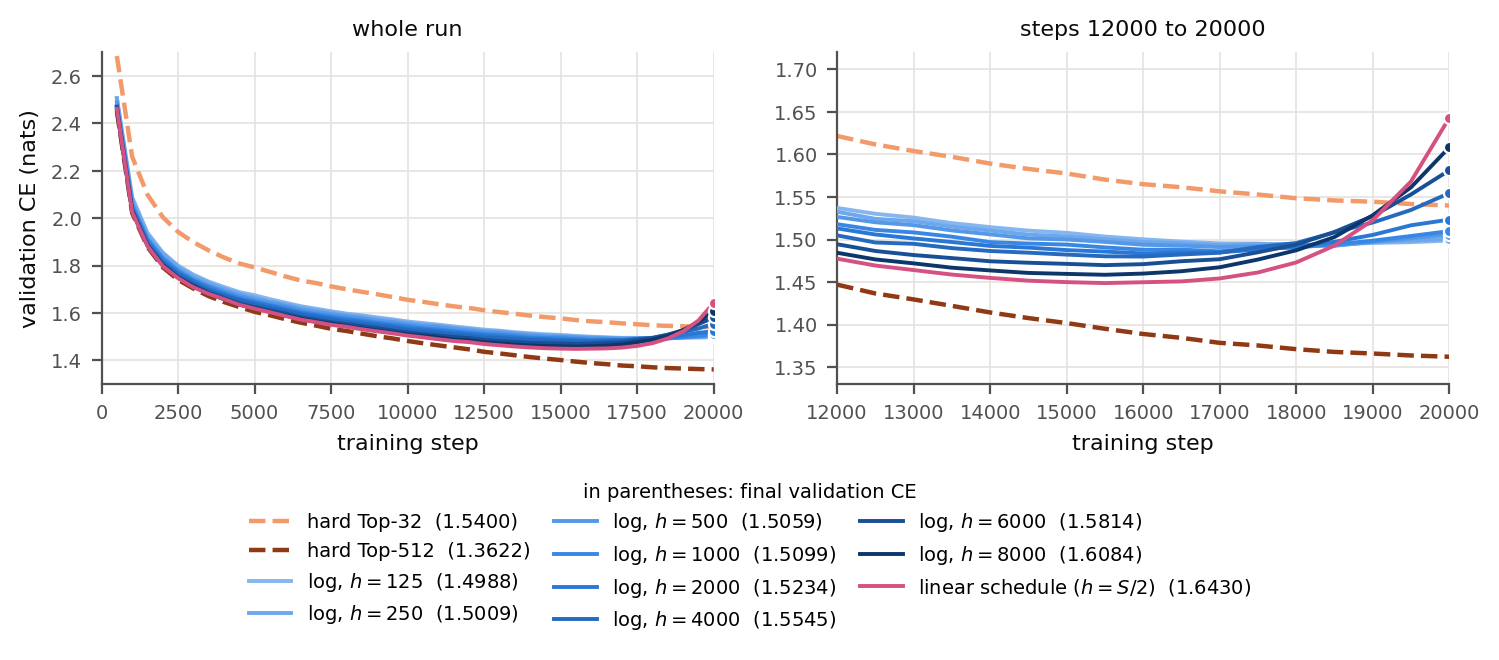
\includegraphics[width=\textwidth]{figures/val_ce.png}
\caption{Validation cross-entropy (the same 960 windows of 512 tokens for every
run, every 500 steps). Dashed: hard Top-32 (light orange) and hard Top-512
(dark orange) at fixed width. Solid: K-annealing from $\Kp = 512$ to $K = 32$: the log schedule in
blue, from light ($h = 125$) to dark ($h = 8000$), and the linear schedule
($h = S/2$) in magenta. The validation loss of an annealed run at step $s$ is measured at
its current width $\Kp(s)$ (Figure~\ref{fig:active}); only its last point
(dot, step 20000) is at $K = 32$ and comparable to hard Top-32. Left: the
whole run; right: steps 12000 to 20000. Legend: final validation CE.}
\label{fig:val}
\end{figure}

\begin{figure}[!htb]
\centering
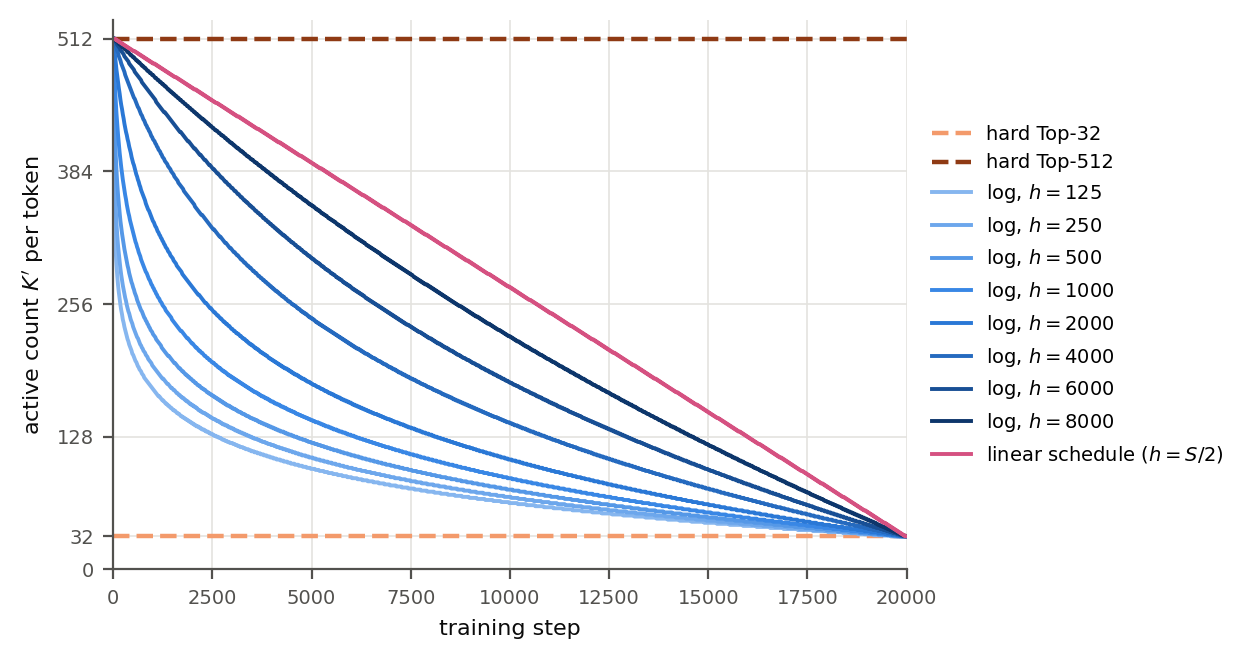
\includegraphics[width=.8\textwidth]{figures/active_count.png}
\caption{Active count $\Kp$ per token at every bottleneck, as logged by each
run (\code{bottleneck/active\_count}, every 20 steps). Colors as in
Figure~\ref{fig:val}; the dashed lines are the fixed widths of the hard
baselines.}
\label{fig:active}
\end{figure}

\begin{figure}[!htb]
\centering
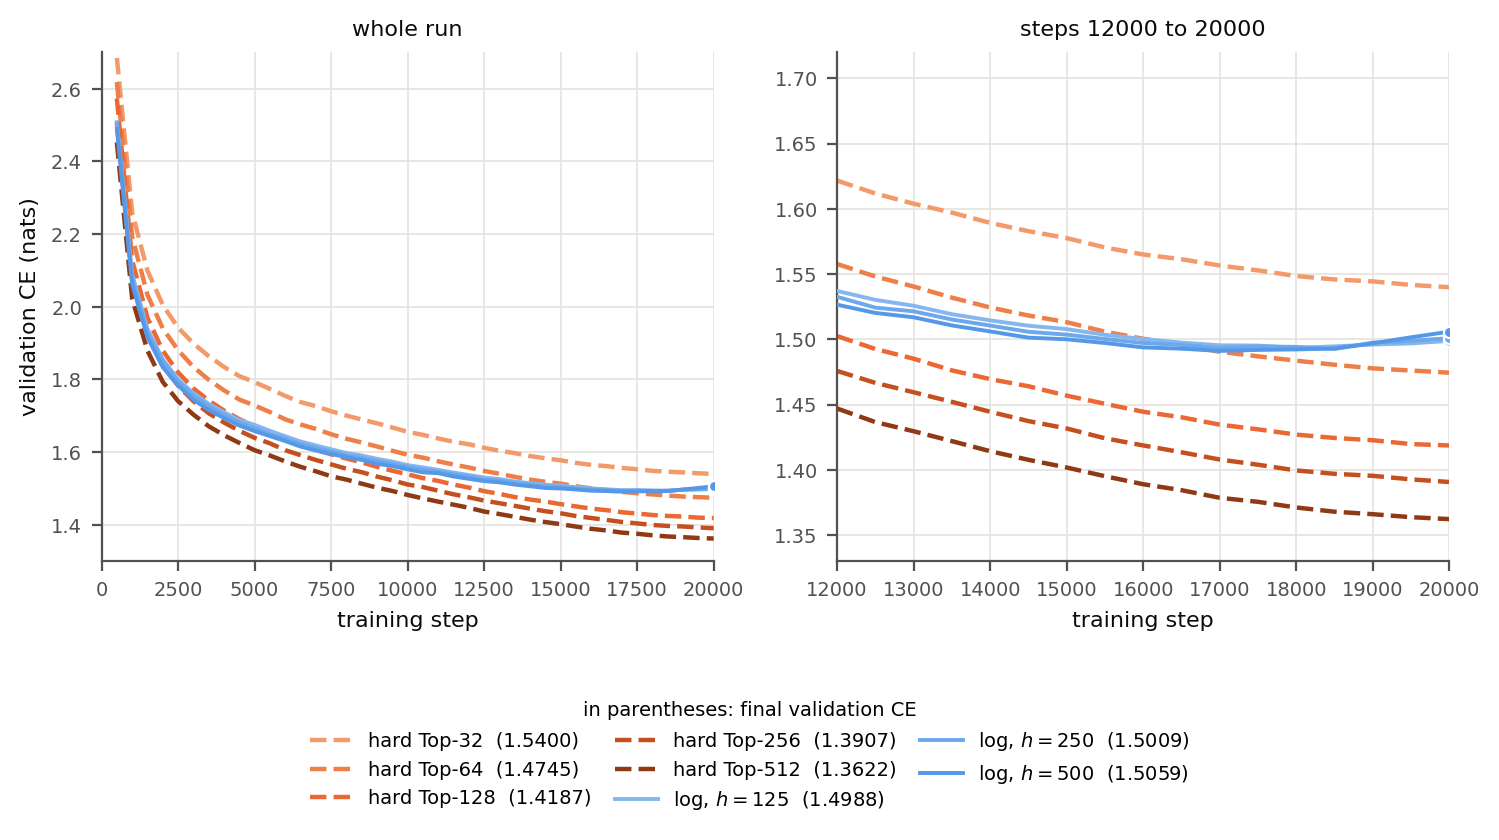
\includegraphics[width=\textwidth]{figures/val_ce_ladder.png}
\caption{Validation cross-entropy of the log schedule at $h = 125$, $250$,
$500$ (solid, blue as in Figure~\ref{fig:val}) against the code-carried hard
Top-$K$ ladder $K = 32, 64, 128, 256, 512$ of
\code{docs/kj-vs-hard-topk-code-residual.tex} (dashed, orange from light to
dark with $K$). The annealed runs are measured at their current width
$\Kp(s)$; only their last point (dot) is at $K = 32$. Left: the whole run;
right: steps 12000 to 20000. Legend: final validation CE.}
\label{fig:ladder}
\end{figure}

\begin{figure}[!htb]
\centering
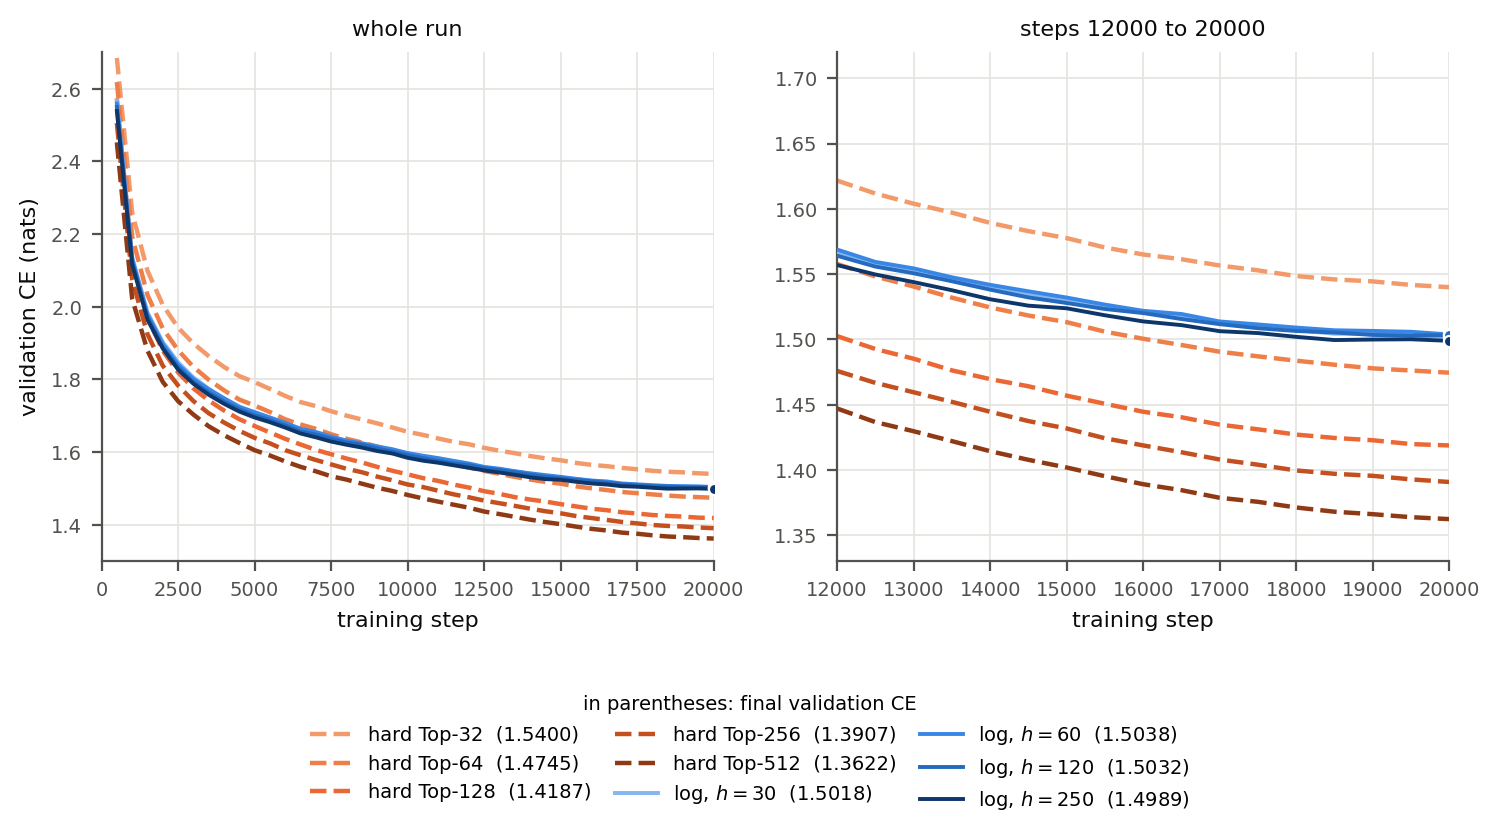
\includegraphics[width=\textwidth]{figures/val_ce_ladder_j224.png}
\caption{As Figure~\ref{fig:ladder} at $J = 224$: the log schedule from
$\Kp = K + J = 256$ to $K = 32$ at $h = 30$, $60$, $120$, $250$ (solid,
blue from light to dark with $h$) against the code-carried hard Top-$K$
ladder (dashed, orange from light to dark with $K$). The annealed runs are
measured at their current width $\Kp(s)$; only their last point (dot) is at
$K = 32$. Left: the whole run; right: steps 12000 to 20000. Legend: final
validation CE.}
\label{fig:ladder224}
\end{figure}

\begin{figure}[!htb]
\centering
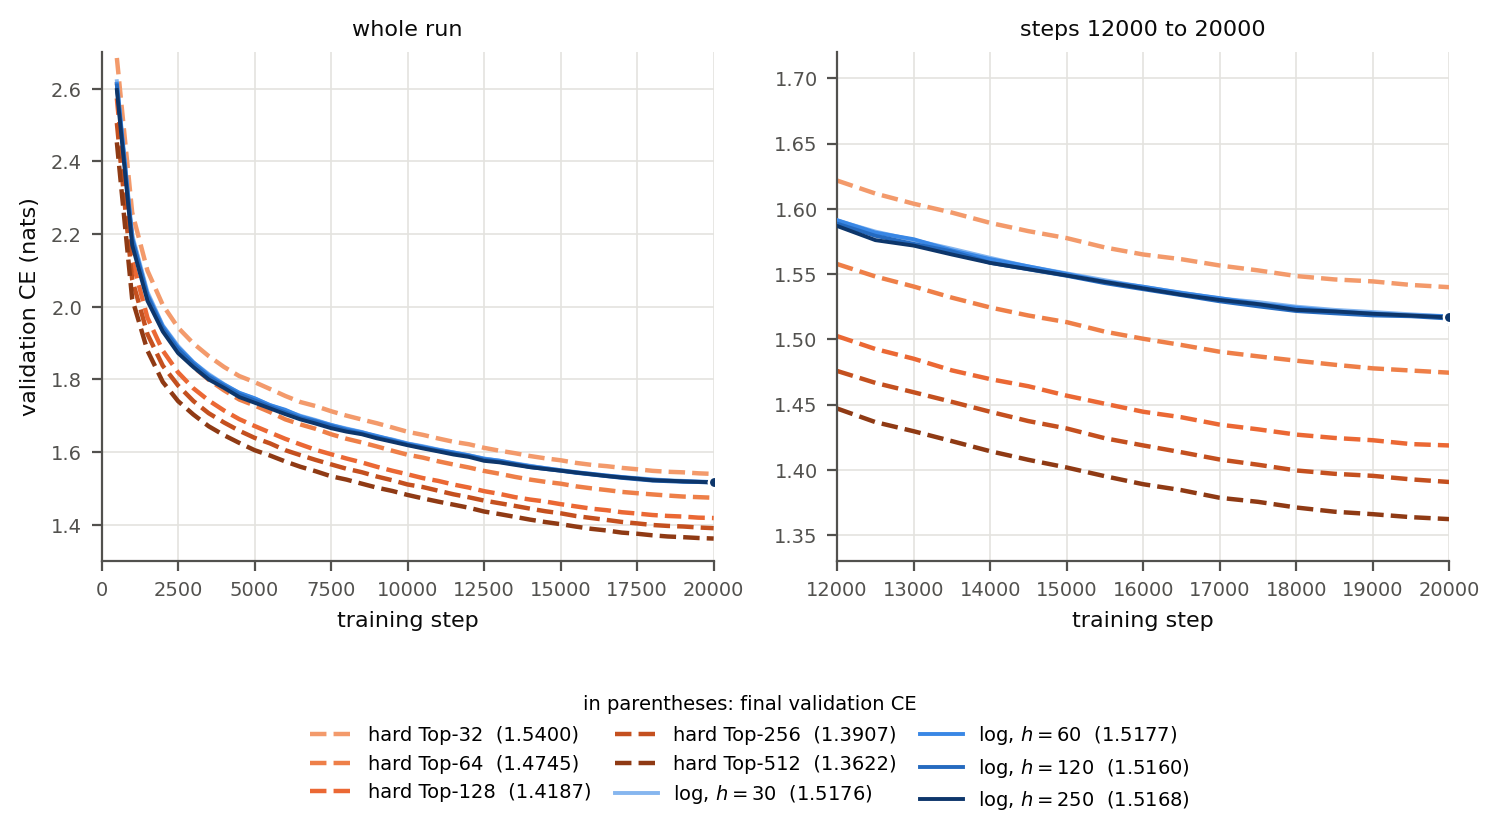
\includegraphics[width=\textwidth]{figures/val_ce_ladder_j96.png}
\caption{As Figure~\ref{fig:ladder} at $J = 96$: the log schedule from
$\Kp = K + J = 128$ to $K = 32$ at $h = 30$, $60$, $120$, $250$ (solid,
blue from light to dark with $h$) against the code-carried hard Top-$K$
ladder (dashed, orange from light to dark with $K$). The annealed runs are
measured at their current width $\Kp(s)$; only their last point (dot) is at
$K = 32$. Left: the whole run; right: steps 12000 to 20000. Legend: final
validation CE.}
\label{fig:ladder96}
\end{figure}

\clearpage
% ============================================================
\section*{Runs}
% ============================================================

All under \code{gdrive:weight-sparsity/}; configs in the repository.

\begin{center}\footnotesize
\begin{tabular}{lll}
\toprule
curve & Drive & config \\
\midrule
hard Top-32  & \code{runs\_madrid/ma\_cr\_hard\_k32\_pnorm}  & \code{configs/cr\_kj/} \\
hard Top-64  & \code{runs\_madrid/ma\_cr\_hard\_k64\_pnorm}  & \code{configs/cr\_kj/} \\
hard Top-128 & \code{runs\_madrid/ma\_cr\_hard\_k128\_pnorm} & \code{configs/cr\_kj/} \\
hard Top-256 & \code{runs\_madrid/ma\_cr\_hard\_k256\_pnorm} & \code{configs/cr\_kj/} \\
hard Top-512 & \code{runs\_madrid/ma\_cr\_hard\_k512\_pnorm} & \code{configs/cr\_kj/} \\
linear, $J = 480$ & \code{runs\_riga/ri\_cr\_hard\_kanneal\_k32\_j480\_pnorm} & \code{configs/hard\_k\_anneal/} \\
log, $J = 480$, $h = 125$ & \code{runs\_tallinn/ta\_cr\_hard\_klog\_h125\_k32\_j480\_pnorm}  & \code{configs/hard\_k\_anneal/} \\
log, $J = 480$, $h = 250$ & \code{runs\_tallinn/ta\_cr\_hard\_klog\_h250\_k32\_j480\_pnorm}  & \code{configs/hard\_k\_anneal/} \\
log, $J = 480$, $h = 500$ & \code{runs\_tallinn/ta\_cr\_hard\_klog\_h500\_k32\_j480\_pnorm}  & \code{configs/hard\_k\_anneal/} \\
log, $J = 480$, $h = 1000$ & \code{runs\_tallinn/ta\_cr\_hard\_klog\_h1000\_k32\_j480\_pnorm} & \code{configs/hard\_k\_anneal/} \\
log, $J = 480$, $h = 2000$ & \code{runs\_tallinn/ta\_cr\_hard\_klog\_h2000\_k32\_j480\_pnorm} & \code{configs/hard\_k\_anneal/} \\
log, $J = 480$, $h = 4000$ & \code{runs\_tallinn/ta\_cr\_hard\_klog\_h4000\_k32\_j480\_pnorm} & \code{configs/hard\_k\_anneal/} \\
log, $J = 480$, $h = 6000$ & \code{runs\_tallinn/ta\_cr\_hard\_klog\_h6000\_k32\_j480\_pnorm} & \code{configs/hard\_k\_anneal/} \\
log, $J = 480$, $h = 8000$ & \code{runs\_tallinn/ta\_cr\_hard\_klog\_h8000\_k32\_j480\_pnorm} & \code{configs/hard\_k\_anneal/} \\
log, $J = 224$, $h = 30$ & \code{runs\_tallinn/ta\_cr\_hard\_klog\_h30\_k32\_j224\_pnorm} & \code{configs/hard\_k\_anneal/} \\
log, $J = 224$, $h = 60$ & \code{runs\_tallinn/ta\_cr\_hard\_klog\_h60\_k32\_j224\_pnorm} & \code{configs/hard\_k\_anneal/} \\
log, $J = 224$, $h = 120$ & \code{runs\_tallinn/ta\_cr\_hard\_klog\_h120\_k32\_j224\_pnorm} & \code{configs/hard\_k\_anneal/} \\
log, $J = 224$, $h = 250$ & \code{runs\_tallinn/ta\_cr\_hard\_klog\_h250\_k32\_j224\_pnorm} & \code{configs/hard\_k\_anneal/} \\
log, $J = 96$, $h = 30$ & \code{runs\_tallinn/ta\_cr\_hard\_klog\_h30\_k32\_j96\_pnorm} & \code{configs/hard\_k\_anneal/} \\
log, $J = 96$, $h = 60$ & \code{runs\_tallinn/ta\_cr\_hard\_klog\_h60\_k32\_j96\_pnorm} & \code{configs/hard\_k\_anneal/} \\
log, $J = 96$, $h = 120$ & \code{runs\_tallinn/ta\_cr\_hard\_klog\_h120\_k32\_j96\_pnorm} & \code{configs/hard\_k\_anneal/} \\
log, $J = 96$, $h = 250$ & \code{runs\_tallinn/ta\_cr\_hard\_klog\_h250\_k32\_j96\_pnorm} & \code{configs/hard\_k\_anneal/} \\
\bottomrule
\end{tabular}
\end{center}

Each run directory holds \code{config.json}, \code{metrics.jsonl},
\code{summary.json}, the TensorBoard events (\code{tb/}) and the checkpoints
every 2000 steps. The figures are drawn by \code{scripts/plot\_kanneal.py}
from \code{docs/kanneal/data/curves.json}, extracted from the runs'
\code{metrics.jsonl}.

\end{document}
